\let\cleardoublepage\clearpage
\chapter{Производственные и обрабатывающие отрасли}

{\bfseries МРНТИ 65.09.05}

\section{СПРОС НАСЕЛЕНИЯ НА ЗЕРНОВЫЕ НАПИТКИ В РК}

\begin{center}
{\bfseries А.Ж.Хастаева*}
\includegraphics[height=1em]{image52},
{\bfseries А.А.Бектурганова}
\includegraphics[height=1em]{image52},
{\bfseries А.М.Омаралиева}
\includegraphics[height=1em]{image52},
{\bfseries А.Ж.Сериков}
\includegraphics[height=1em]{image52},
{\bfseries Р.К.Суюндык}

Казахский университет технологии и бизнеса, Астана, Казахстан,

e-mail: gera\_or@mail.ru
\end{center}

Сегмент молочных альтернатив продолжает активно развиваться.
Растительные напитки больше не являются просто данью моде или продуктом
для узкого круга последователей вегетарианства. Интерес к категории со
стороны традиционных производителей молочной продукции является
наглядным подтверждением того, что направление вышло за рамки нишевого
бизнеса и может конкурировать даже с обычным молоком.

{\bfseries Ключевые слова:} растительное молоко, омега-3, потребитель,
опрос.

\begin{center}
{\large\bfseries ҚАЗАҚСТАН РЕСПУБЛИКАСЫНДАҒЫ АСТЫҚ СУСЫНДАРЫНА ХАЛЫҚТЫҢ СҰРАНЫСЫ}

\vspace{1em}
{\bfseries А.Ж.Хастаева*}
\includegraphics[height=1em]{image52},
{\bfseries А.А.Бектурганова}
\includegraphics[height=1em]{image52},
{\bfseries А.М.Омаралиева}
\includegraphics[height=1em]{image52},
{\bfseries А.Ж.Сериков}
\includegraphics[height=1em]{image52},
{\bfseries Р.К.Суюндык}

Қазақ технология және бизнес университеті, Астана, Қазақстан,

e-mail: gera\_or@mail.ru
\end{center}

Сүт баламаларының сегменті белсенді дамуын жалғастыруда. Өсімдік
негізіндегі сусындар енді сәнге немесе вегетариандық ізбасарлардың тар
шеңберіне арналған өнім емес. Дәстүрлі сүт өндірушілерінің санатқа деген
қызығушылығы бұл бағыттың тауашалық бизнестен тыс болғанын және тіпті
қарапайым сүтпен бәсекеге түсе алатындығының айқын дәлелі болып
табылады.

{\bfseries Түйін сөздер:} өсімдік сүті, омега-3, тұтынушы, сауалнама.

\begin{center}
{\large\bfseries POPULATION DEMAND FOR VEGETABLE DRINKS IN THE REPUBLIC OF
KAZAKHSTAN}

\vspace{1em}
{\bfseries А.Zh.Khastayeva*}
\includegraphics[height=1em]{image52},
{\bfseries A.A. Bekturganova}
\includegraphics[height=1em]{image52},
{\bfseries A. M. Omaraliyeva}
\includegraphics[height=1em]{image52},
{\bfseries A.Zh.Serikov}
\includegraphics[height=1em]{image52},
{\bfseries R.K.Suyundyk}

Kazakh University of Technology and Business, Astana, Republic of
Kazakhstan,

e-mail: gera\_or@mail.ru
\end{center}

The segment of dairy alternatives continues to develop actively. Herbal
drinks are no longer just a fashion statement or a product for a narrow
circle of vegetarian followers. Interest in the category from
traditional dairy producers is a clear confirmation that the direction
has gone beyond the niche business and can even compete with regular
milk.

{\bfseries Keywords:} vegetable milk, omega-3, consumer, survey.

\begin{multicols}{2}
{\bfseries Введение.} Активное развитие производства растительного молока
связано с индивидуальной непереносимостью лактозы или молочного казеина
и активной пропагандой вегетарианства, а также с физиологическими
преимуществами потребления растительного белка, особенно с
геродиетическим питанием {[}1-5{]}.

В настоящее время разработаны функциональные пищевые продукты, в состав
которых входят биологически активные соединения, выделенные из растений,
полиненасыщенные жирные кислоты, пробиотики, пребиотики, минералы и
витамины {[}6-9{]}.

По прогнозам аналитиков международного рынка в 2022 году рынок
растительных заменителей молока вырос до 9 млрд. \$. В год площадка по
производству растительного молока будет прибавлять по 7,1\% в
стоимостном выражении. За пять лет продажи в сегменте производства
растительных напитков выросли на 61\%, в то время как показатели
коровьего молока, напротив, снизились на 15\% {[}10-12{]}.

Необходимо отметить, что анализ существующего рынка растительного
молока, а также маркетинговые исследования вносят существенный вклад в
развитие производства данной продукции.

Для разработки новой технологии важно знать предпочтения населения в
потреблении той или иной группы товаров, особенно это важно для рынка
напитков функционального назначения, насчитывающего большое разнообразие
ассортимента.

{\bfseries Материалы и методы.} Нами проведен социологический опрос методом
онлайн - анкетирования, на основании чего проанализирован спрос на
растительные напитки среди населения разных возрастов, изучены
потребности жителей Казахстана в растительных напитках.

Представленная для опроса анкета состояла из 15 вопросов. Вопросы анкеты
раскрывают возраст и пол участников, частоту употребляемости
растительных напитков, каким продуктам и производителям они отдают
предпочтение, а также какую еще продукцию хотят увидеть в будущем на
рынке Казахстана.

{\bfseries Результаты и обсуждение.} В результате анкетировнаия были
получены анкеты от 317 респондентов из различных регионов Казахстана.

Вопросы анкеты были составлены с учетом тенденций, наблюдающихся в
развитии производства новых видов напитков из зерновых культур.
Известно, что в последнее время происходит постепенный отказ от
использования искусственных пищевых добавок, что связано со сменой
приоритетов со стороны потребителей, которые все больше заботятся о
своем здоровье и предпочитают покупать натуральные и полезные для
организма продукты или делают выбор в пользу низкокалорийных продуктов.
У некоторой части категории граждан улучшается материальное положение,
и, как следствие, возрастают требования к употребляемым продуктам
питания с учетом того, что регулярный вывод на рынок новинок, в том
числе с новыми вкусовыми сочетаниями, оригинальной рецептурой является
еще одной важной тенденцией последних лет.

Большую часть опрошенных респондентов составили девушки и юноши в
возрасте от 18 до 30 лет, также значительный сегмент занимали
респонденты от 30 до 40 и от 40 до 50 лет в соответствии с рисунком 1.
\end{multicols}

\begin{figure}[htbp]
\begin{subfigure}[b]{0.45\textwidth}
\centering
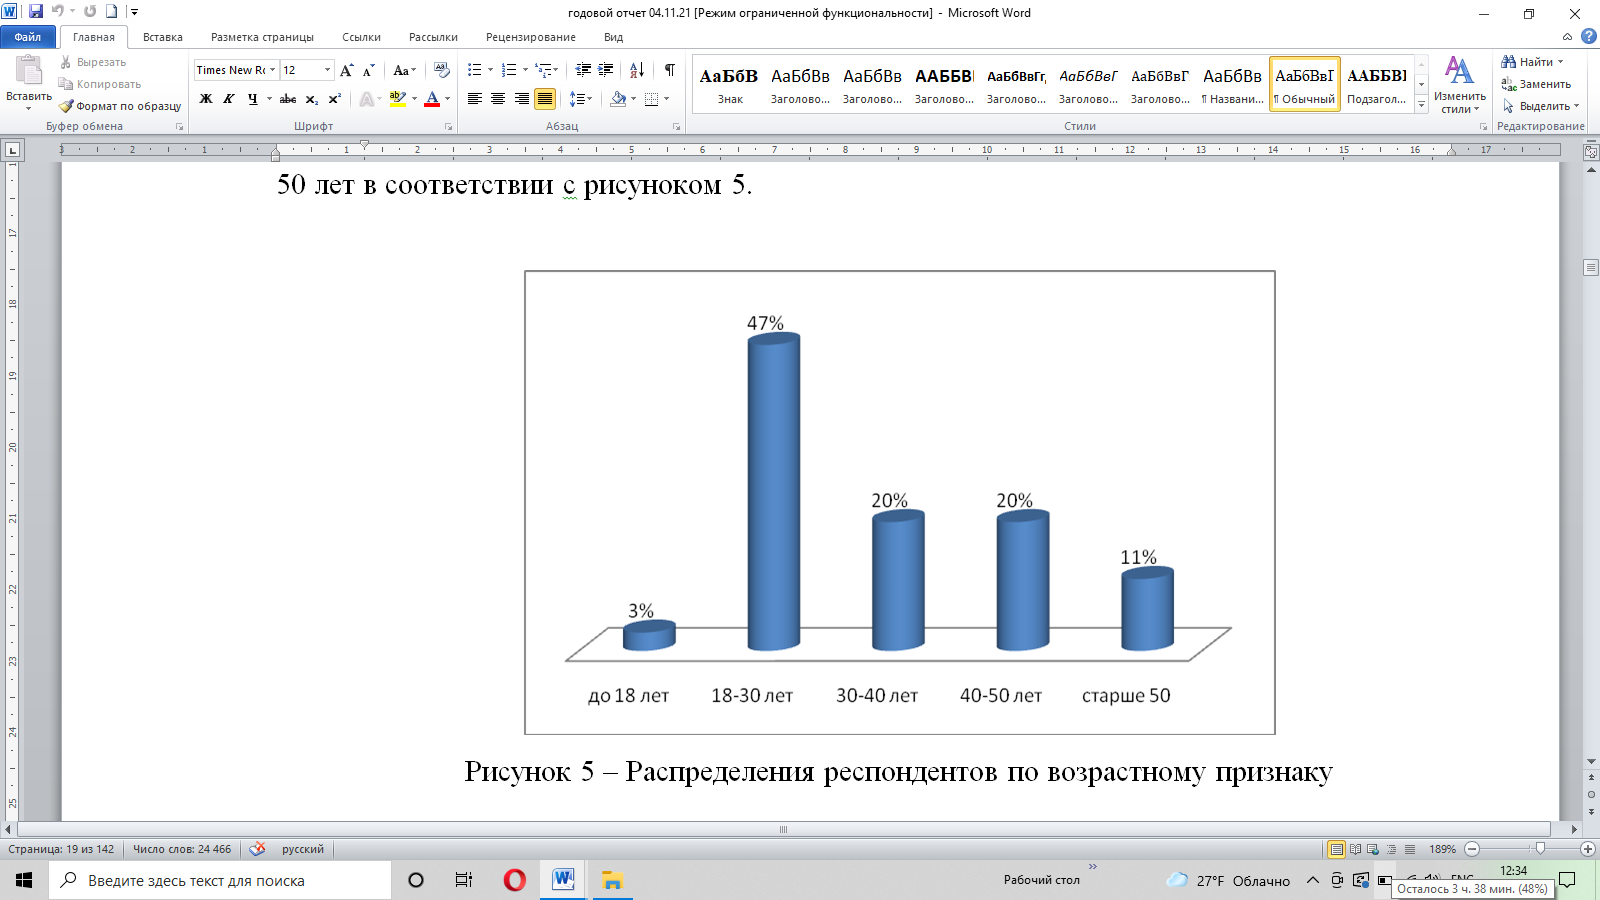
\includegraphics[width=\textwidth]{image53}
\caption*{Рис. 1 - Распределения респондентов по возрастному признаку}
\end{subfigure}
\hspace{0.05\textwidth}
\begin{subfigure}[b]{0.45\textwidth}
\centering
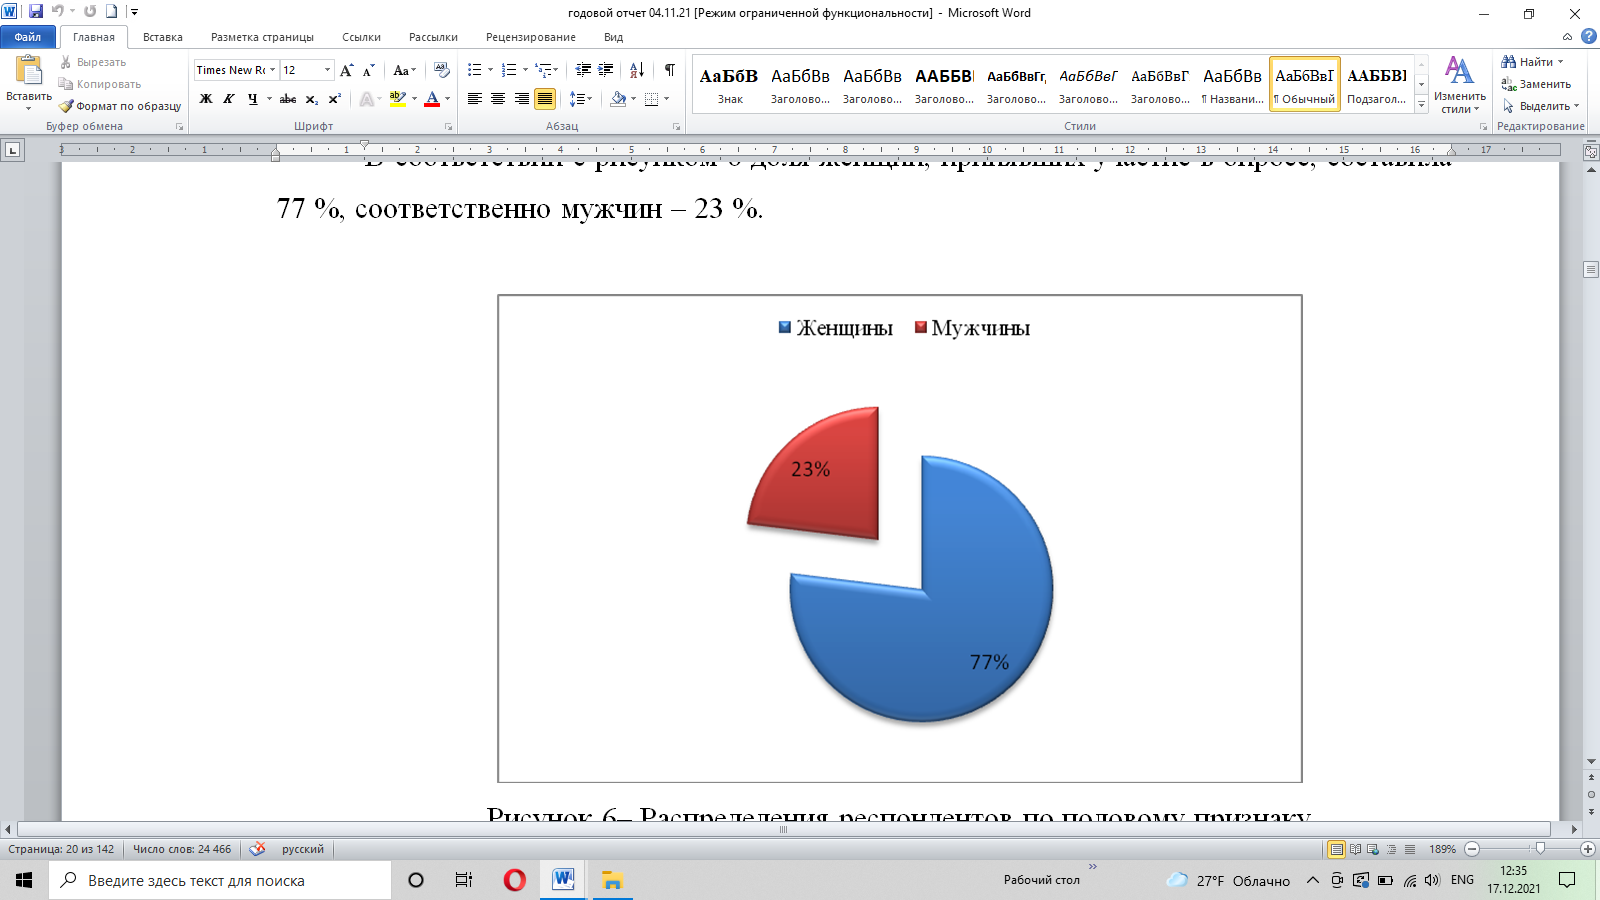
\includegraphics[height=\textwidth]{image54}
\caption*{Рис. 2 - Распределения респондентов по половому признаку}
\end{subfigure}
\end{figure}

В соответствии с рисунком 2 доля женщин, принявших участие в опросе,
составила 77 \%, соответственно мужчин - 23 \%.

Анализ результатов опроса выявил, что большинство (23,1\%) употребляют
растительное молоко не реже 4-х раз в неделю. Так же, что 20,80\%
респондентов предпочитают употреблять растительное молоко 1-2 раза в
неделю (рисунок 3). Учитывая также, что более 11,60\% опрошенных
потребляют данный вид продукции ежедневно, можно говорить о значительной
роли растительного молока в питании потребителей.

\begin{figure}[htbp]
\begin{subfigure}[b]{0.45\textwidth}
\centering
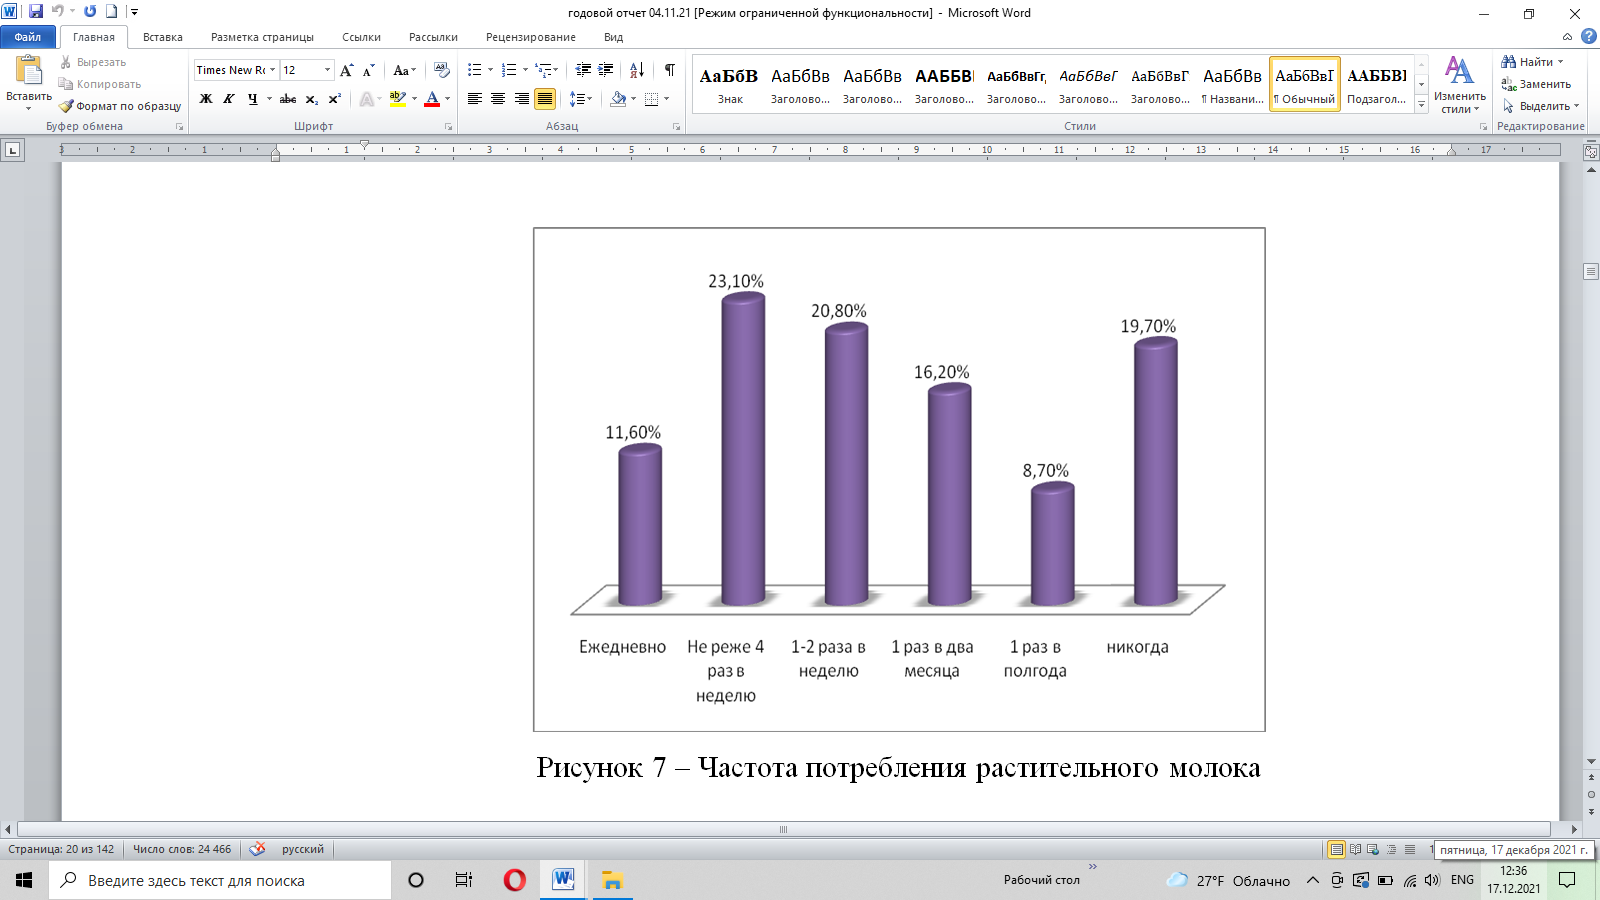
\includegraphics[width=\textwidth]{image55}
\caption*{Рис. 3 - Частота потребления растительного молока}
\end{subfigure}
\hspace{0.05\textwidth}
\begin{subfigure}[b]{0.45\textwidth}
\centering
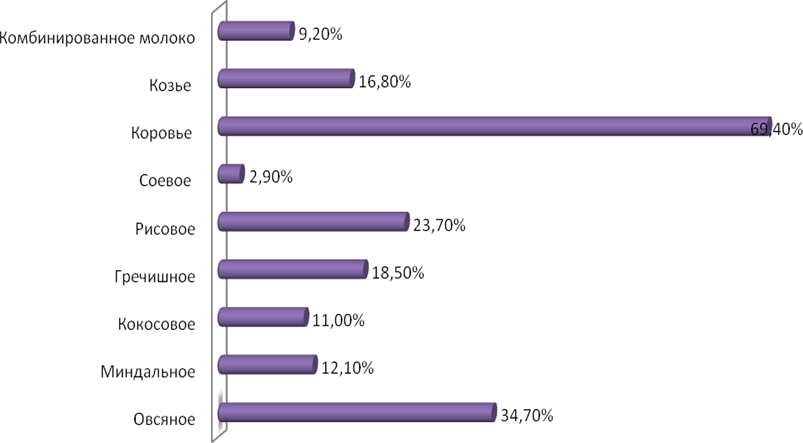
\includegraphics[width=\textwidth]{image56}
\caption*{Рис. 4 - Предпочтений разных видов молока в будни}
\end{subfigure}
\end{figure}

Лидером по употреблению молока в будни является коровье питьевое молоко
(более 69,4\%). Около 34,7\% опрошенных предпочитали овсяное молоко,
более 23,7\% респондентов назвали рисовое молоко в качестве ежедневно
употребляемого продукта (рисунок 4).

На вопрос, «С какой целью вы покупаете растительное молоко?» 43,40\%
респондентов ответили, что у них интерес к новым продуктам; 26,6\%
опрошенных ответили, что употребляют растительное молоко с чаем/кофе,
34,7\% потребителей употребляют растительное молоко, в связи с тем, что
придерживаются принципам правильного питания. 31,8\% респондентов
употребляют растительное молоко, как самостоятельный продукт, и у 6,9\%
опрошенных имеется не переносимость лактозы (рисунок 5).

\begin{figure}[htbp]
\begin{subfigure}[b]{0.45\textwidth}
\centering
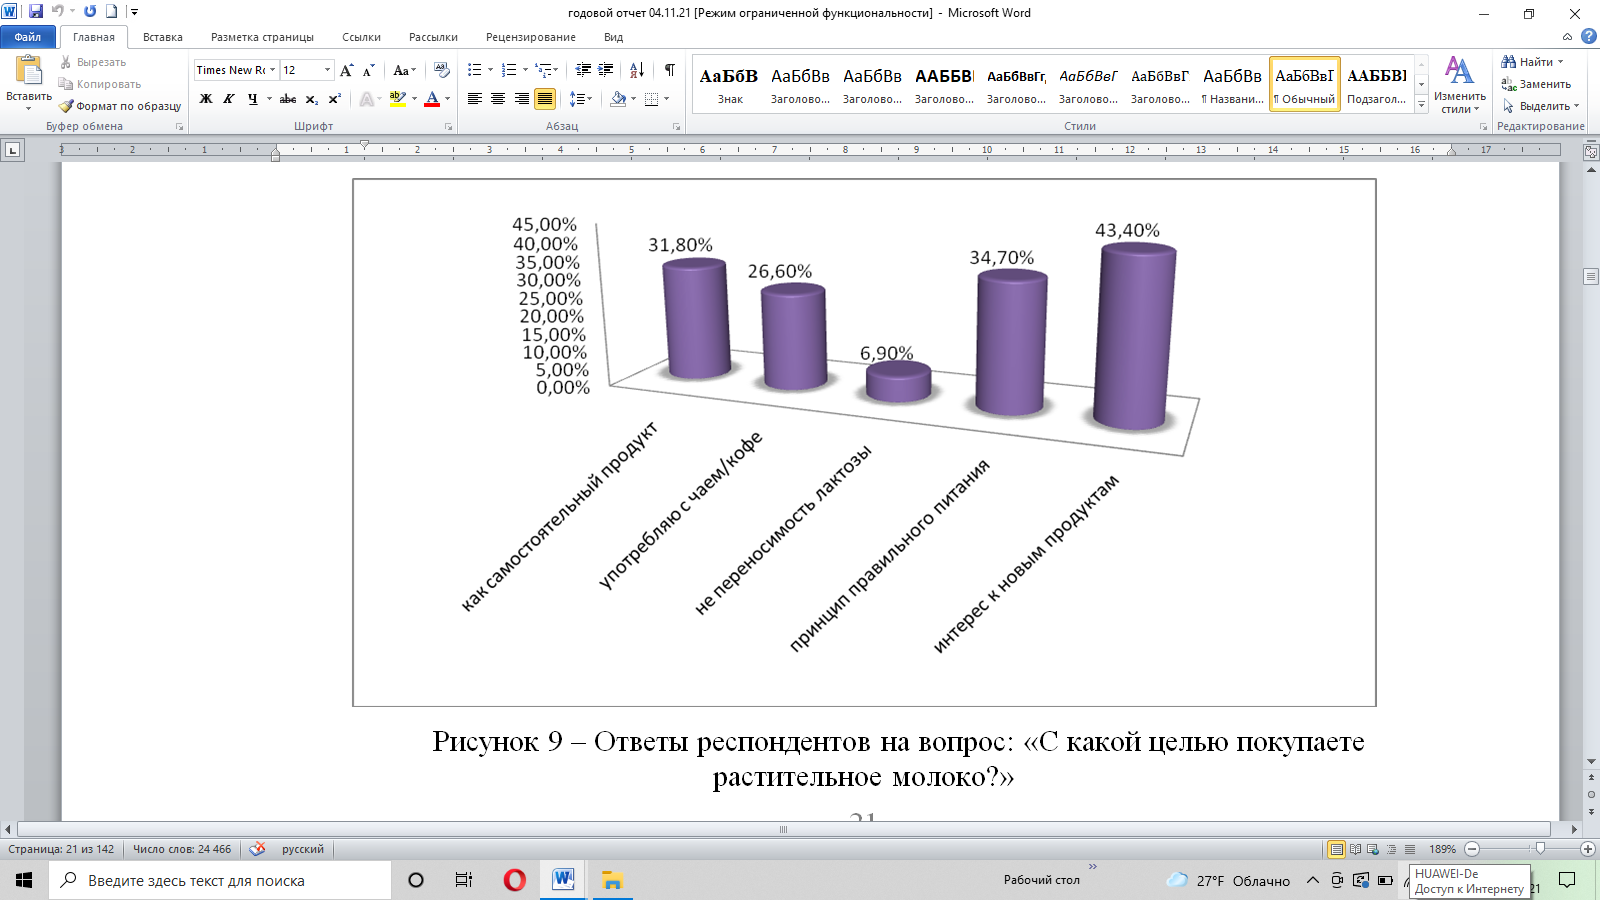
\includegraphics[width=\textwidth]{image57}
\caption*{Рис. 5 - Ответы респондентов на вопрос: «С какой целью покупаете растительное молоко?»}
\end{subfigure}
\hspace{0.05\textwidth}
\begin{subfigure}[b]{0.45\textwidth}
\centering
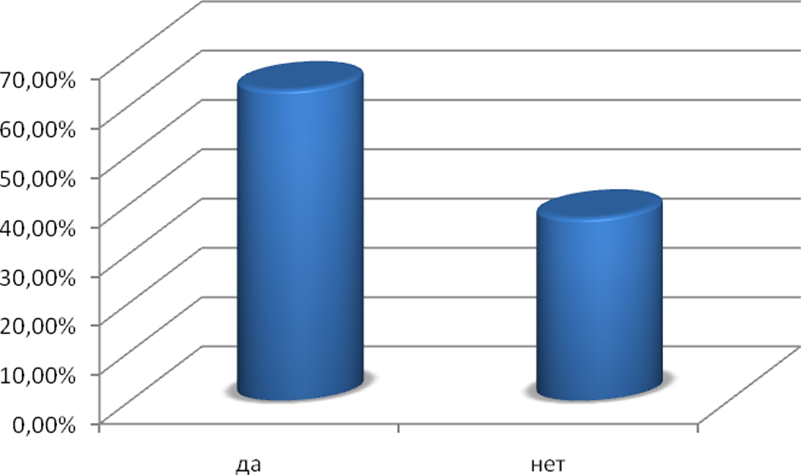
\includegraphics[width=\textwidth]{image58}
\caption*{Рис. 6 - Ответы на вопрос: «Покупаете ли вы растительное молоко?»}
\end{subfigure}
\end{figure}

На вопрос, «Покупаете ли вы растительное молоко?» большая часть
опрошенных ответили положительно (63\%) (рисунок 6).

При выборе растительного молока как для женщин, так для мужчин
(независимо от возраста) наиболее важным критерием являются качество
продукта (57,8\%). Часть потребителей отметили важным критерием
натуральность ингредиентов (50,3\%), в то время как известность марки
практически не играет роли (не более 6,9\%) (рисунок 7).

\begin{figure}[htbp]
\begin{subfigure}[b]{0.45\textwidth}
\centering
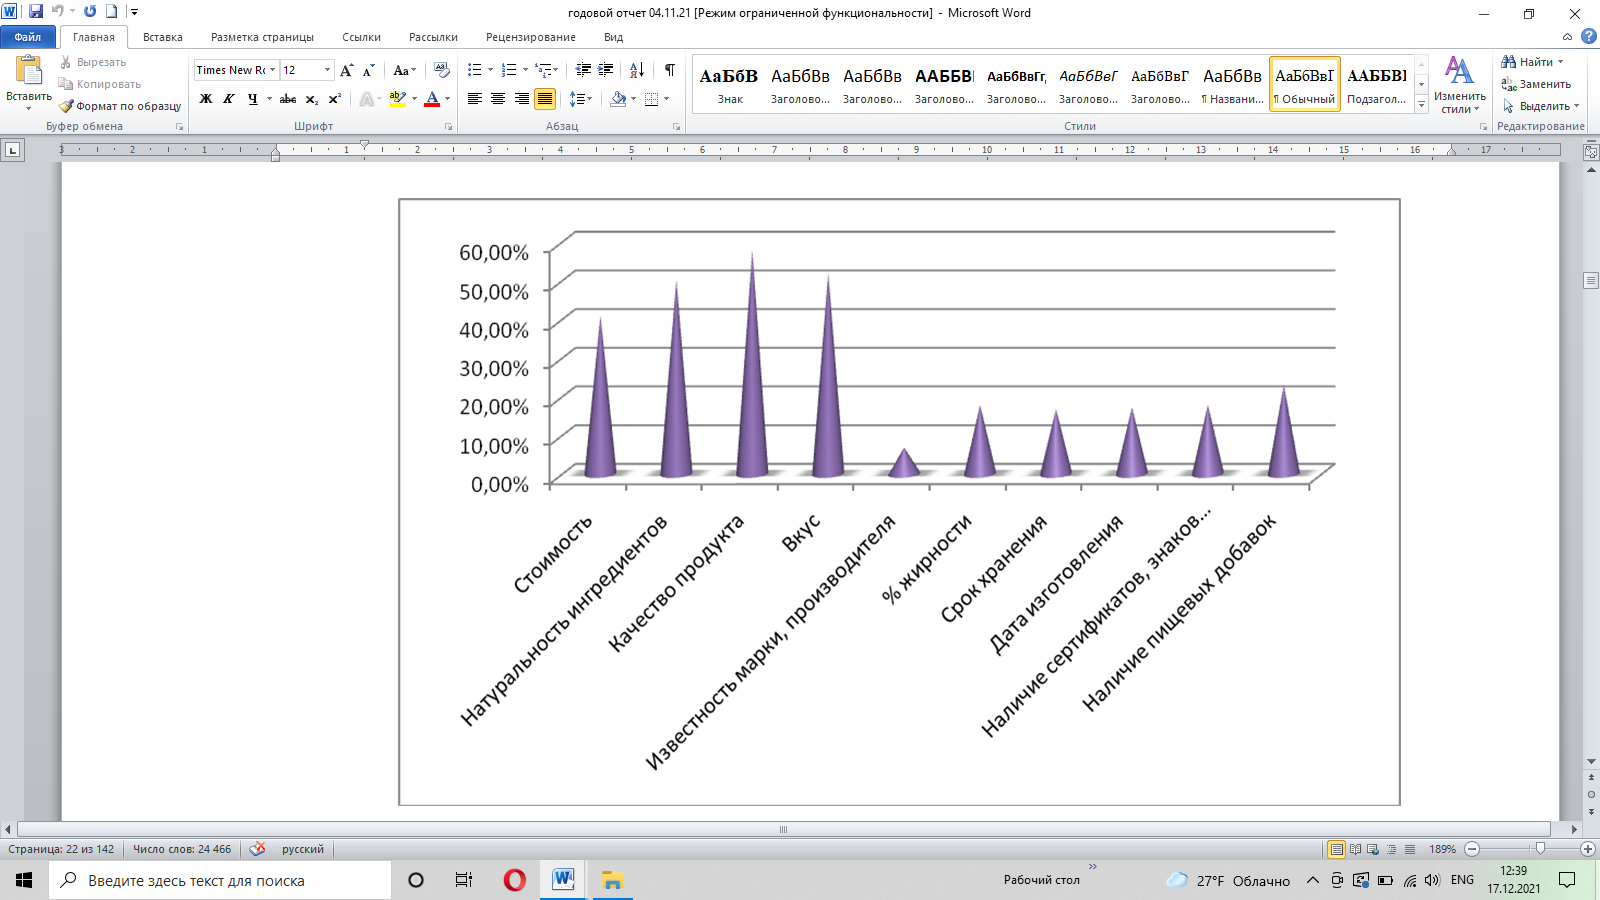
\includegraphics[width=\textwidth]{image59}
\caption*{Рис. 7 - Критерий выбора растительного молока}
\end{subfigure}
\hspace{0.05\textwidth}
\begin{subfigure}[b]{0.45\textwidth}
\centering
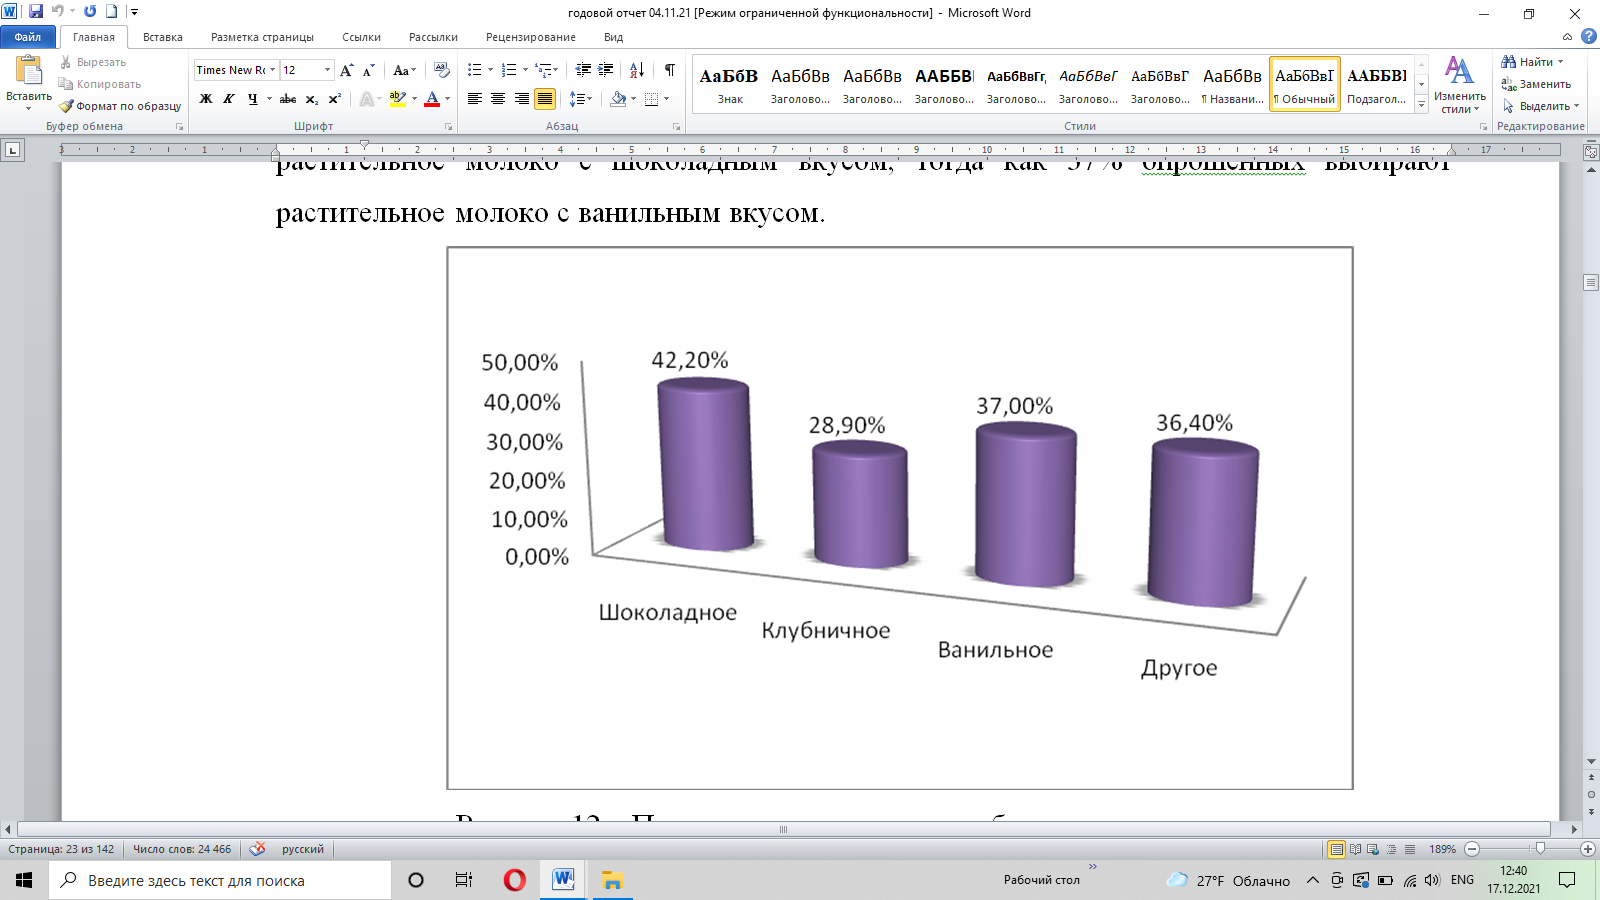
\includegraphics[width=\textwidth]{image60}
\caption*{Рис. 8 - Предпочтения вкуса при выборе растительного молока}
\end{subfigure}
\end{figure}

В соответствии с рисунком 8, 42,2\% респондента предпочитают употреблять
растительное молоко с шоколадным вкусом, тогда как 37\% опрошенных
выбирают растительное молоко с ванильным вкусом.

36,4\% респондентов считают, что ассортимент растительного молока
недостаточно широким, в то время как 15,6\% потребителей считают выбор
растительного молока достаточно широким. 23,1\% опрошенных воздержались,
в связи с тем, что затруднялись ответить (рисунок 9).

\begin{figure}[H]
\begin{subfigure}[b]{0.45\textwidth}
\centering
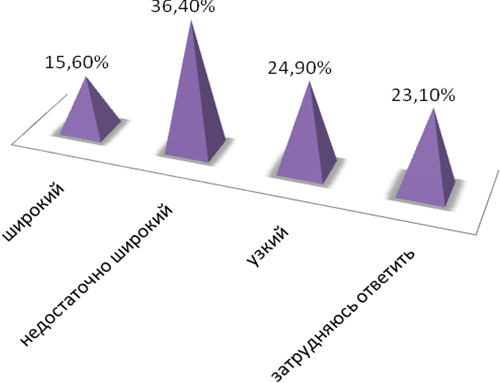
\includegraphics[width=\textwidth]{image61}
\caption*{Рис. 9 - Широта ассортимента растительного молока}
\end{subfigure}
\hspace{0.05\textwidth}
\begin{subfigure}[b]{0.45\textwidth}
\centering
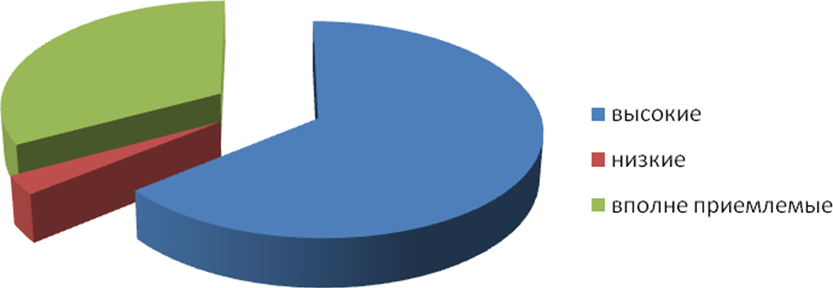
\includegraphics[width=\textwidth]{image62}
\caption*{Рис. 10 - Ценовой сегмент на растительное молоко}
\end{subfigure}
\end{figure}

На вопрос «Как вы считаете, в данный момент цены на растительное молоко»
64,2\% респондентов ответили, что цены на растительное молоко высокие;
32,9\% опрошенных считают, что цены на растительное молоко вполне
приемлемые, и только - 2,9\% респондентов считают, что цены на цены на
растительное молоко низкие (рисунок 10).

На вопрос «Вы хотели бы, чтобы растительное молоко обогащали
Омега-3-полиненысыщенными жирными кислотами?», 90\% респондентов
ответили положительно (рисунок 11).

\begin{figure}[H]
\begin{subfigure}[b]{0.45\textwidth}
\centering
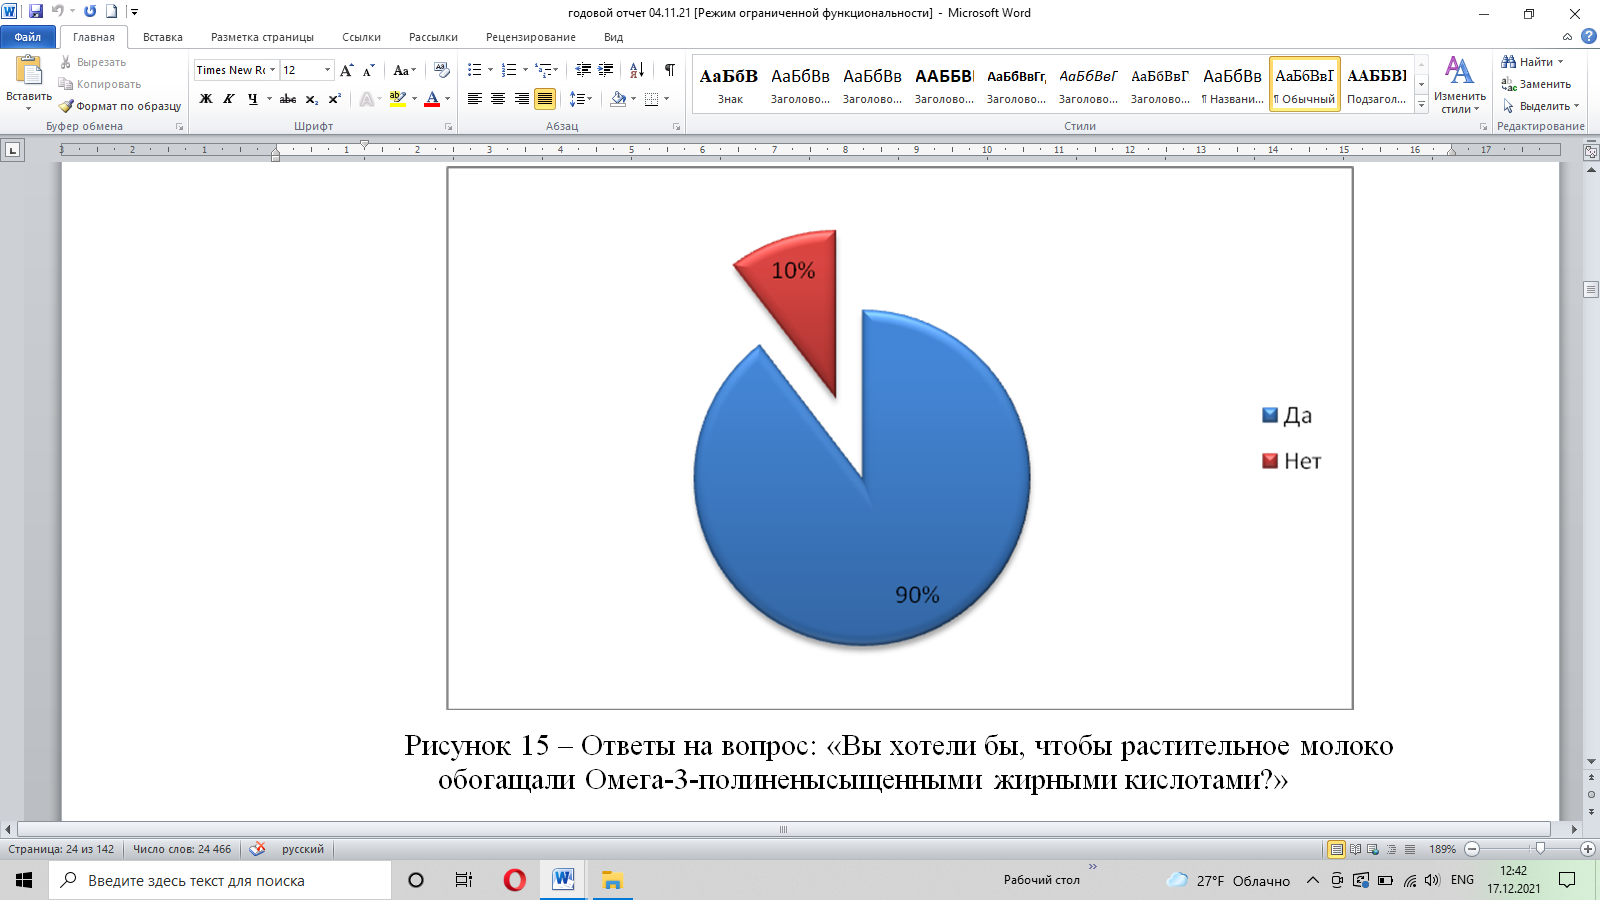
\includegraphics[width=\textwidth]{image63}
\caption*{Рис. 11 - Ответы на вопрос: «Вы хотели бы, чтобы растительное молоко
обогащали Омега-3-полиненысыщенными жирными кислотами?»}
\end{subfigure}
\hspace{0.05\textwidth}
\begin{subfigure}[b]{0.45\textwidth}
\centering
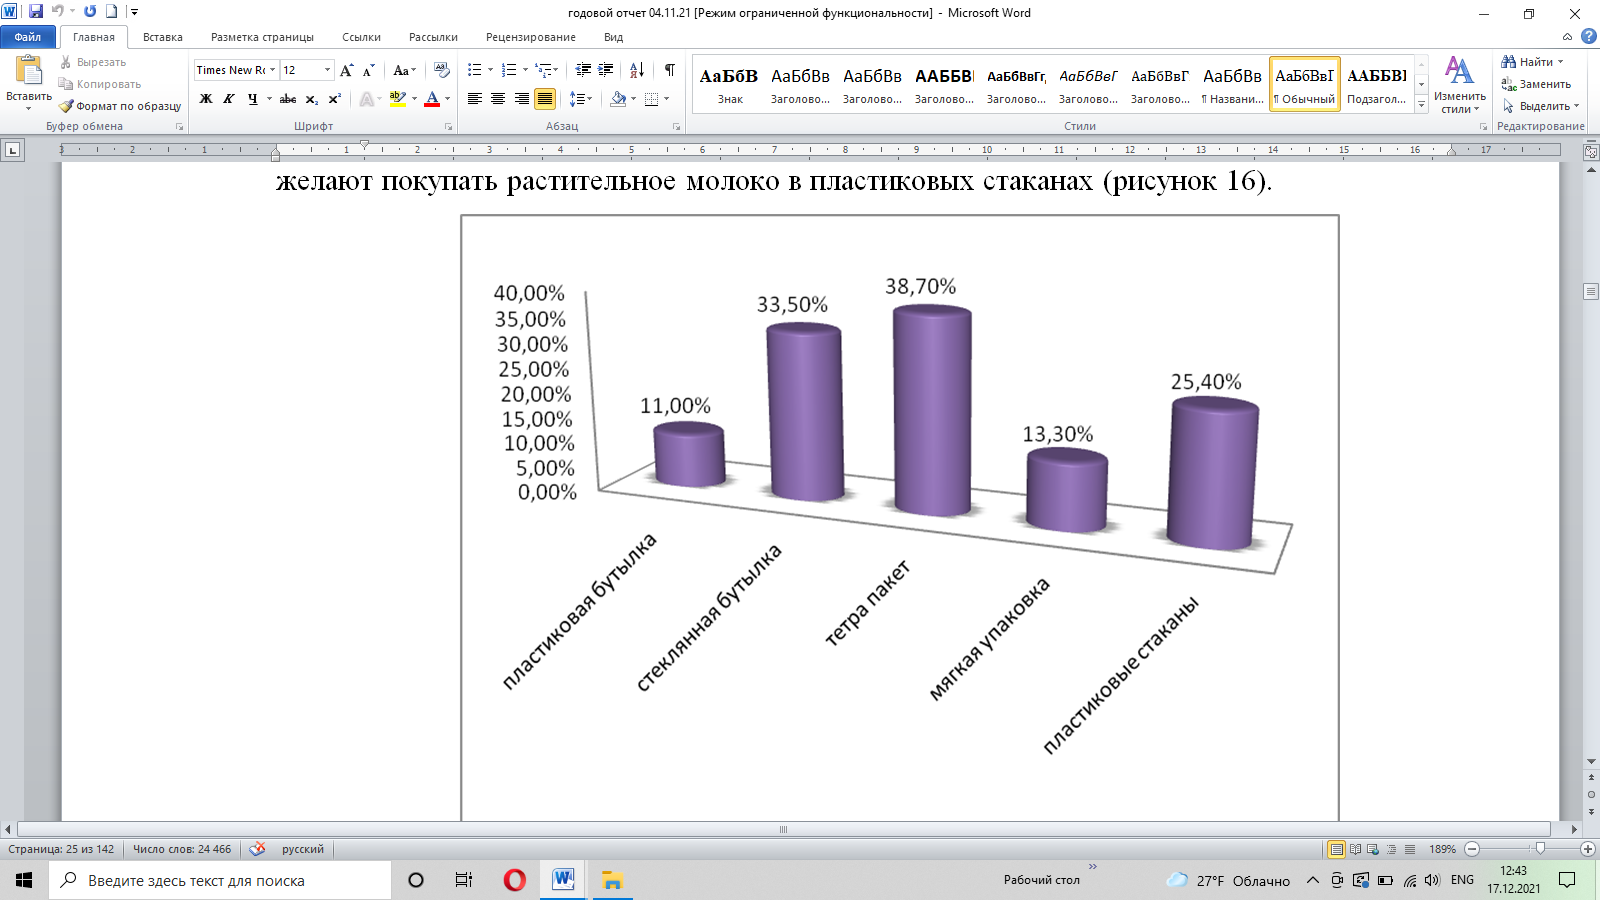
\includegraphics[width=\textwidth]{image64}
\caption*{Рис. 12 - Ответы респондентов на вопрос: «В какой упаковке вы обычно предпочитаете растительное молоко?»}
\end{subfigure}
\end{figure}

\begin{figure}
\centering
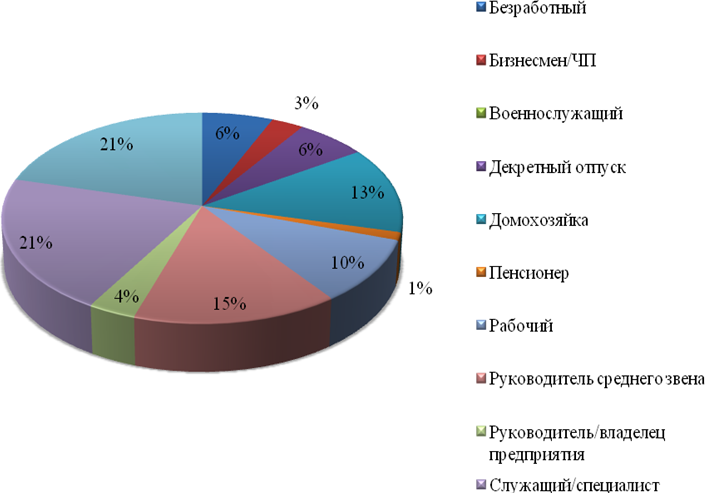
\includegraphics[width=0.8\textwidth]{image65}
\caption*{Рис. 13 - Ценовой сегмент на растительное молоко}
\end{figure}

\begin{multicols}{2}
Большинство опрошенных (38,7\%) предпочитают, чтобы растительное молоко
упаковывали в тетра пакетах, тогда как 33,5\% респондентов желают
покупать растительное молоко в стеклянных бутылках, соответственно,
только 25,40\% потребителей желают покупать растительное молоко в
пластиковых стаканах (рисунок 12).
Так же благодаря опросу мы смогли выяснить основной контингент
потребителей. В числе тех, кто часто употребляет растительное молоко,
это служащий либо специалисты (21\%). 21,8\% студентов являются
потребителями растительного молока. У руководителей среднего звена
(15\%); домохозяек (13,3\%); рабочих (9,8\%) в рационе также
используется растительное молоко (рисунок 13).

В опросе участвовали жители всей республики, но большая часть
респондентов из г.Нур-Султан (42,2\%); г.Алматы (17,3\%); г.Шымкент
(14,5\%); Павлодарской области (5,2\%) и Акмолинской области так же
(5,2\%).

Таким образом, по результатом проведенного социологического опроса
сделан вывод, что около 42,2\% респондентов предпочитают растительное
молоко с шоколадным вкусом, такие критерии, как натуральность продуктов
важны для 50,3\%, цена - для 41\%, \% жирности - для 17,9\%.

В дальнейшем опрос показал, что 89,6\% респондентов готовы употреблять
растительное молоко, если бы они были дополнительно обогащены
Омега-3-полиненысыщенными жирными кислотами. Около 43,4\% опрошенных
стремятся покупать новые изделия, поэтому производство растительного
молока, обогащенных Омега-3 полиненасыщенными жирными кислотами, должно
явиться одним из приоритетов предприятий пищевой и перерабатывающей
промышленности при разработке продуктов массового потребления.

{\bfseries Выводы.} Проведен социологический опрос методом
онлайн-анкетирования, на основании чего проанализирован спрос на
растительные напитки среди населения разных возрастов, изучены
потребности жителей Казахстана в растительных напитках. В результате
анкетирования были получены анкеты от 317 респондентов из различных
регионов Казахстана.
\end{multicols}

\emph{Научно-исследовательская работа выполняется в рамках ПЦФ
Министерством сельского хозяйства Республики Казахстан BR10764970 по
теме «Разработка наукоемких технологий глубокой переработки с/х сырья в
целях расширения ассортимента и выхода готовой продукции с единицы
сырья, а также снижения доли отходов в производстве продукции» на
2021-2023 гг}.

\begin{center}
{\bfseries Литература}
\end{center}

\begin{enumerate}
\item
Будько, Д. Мировой рынок альтернативных молочных продуктов: ожидается
стремительный рост / Д. Будько // Бизнес пищевых ингредиентов.
Апрель-май 2016 {[}Текст{]}. - Режим доступа:
\href{https://novaprodukt.ru/ing/articles/non\_dairy\_milk/}{https://novaprodukt.ru}.

\item
Settaluri, V.S. Peanuts and their nutritional aspects - a review /
V.S. Settaluri, C.V.K. Kandala, N. Puppala, J. Sundaram // Food and
Nutrition Sci-ences. - 2012. - V. 3. - No. 12.- P. 1644-1650, doi:
10.4236/fns.2012.312215.

\item
Sethi, S. Plant-based milk alternatives an emerging segment of
functional beverages: a review / S. Sethi, S.K. Tyagi, R.K. Anurag //
Journal of Food Science and Technology. - 2016. - V. 53. - Iss. 9. -
P. 3408-3423, doi:10.1007/s13197-016-2328-3.

\item
Samofalova, L.A. Scientific justification of the use of germinating
seeds of dicotyledonous plants in the production of plant bases and
substitutes for dairy products of functional significance: abstract.
diss. ... Doctor of Technical Sciences: 05.18.07 / L.A. Samofalova. -
St. Petersburg, 2010 - 32 p.

\item
Makinen, O.E. Foods for special dietary needs: non-dairy plant-based
milk substitutes and fermented dairy-type products / O.E. Makinen, V.
Wanhalinna, E. Zannini, E.K. Arendt // Critical Reviews in Food Science
and Nutrition. - 2016. - V. 56 (3). - P. 339-49,
doi:10.1080/10408398.2012.761950.

\item
Gouw, V.P.; Jung, J.; Zhao, Y. Functional properties, bioactive
compounds, and in vitro gastrointestinal digestion study of dried fruit
pomace powders as functional food ingredients. LWT Food Sci. Technol.
2017, 80, 136-144.

\item
Rathore, S.; Salmeron, I.; Pandiella, S.S. Production of potentially
probiotic beverages using single and mixed cereal substrates fermented
with lactic acid bacteria cultures. Food Microbiol. 2012, 30, 239-244.

\item
Vieira da Silva, B.; Barreira, J.C.M.; Oliveira, M.B.P.P. Natural
phytochemicals and probiotics as bioactive ingredients for functional
foods: Extraction, biochemistry and protected-delivery technologies.
Trends Food Sci. Technol. 2016, 50, 144-158.

\item
Yasmin, A.; Butt, M.S.; van Baak, M.; Shahid, M.Z. Supplementation of
prebiotics to a whey-based beverage reduces the risk of
hypercholesterolaemia in rats. Int. Dairy J. 2015, 48, 80-84.

\item
\href{https://milknews.ru/longridy/rastitelniye-analogi-moloka.html}{https://milknews.ru}

\item
Hambleton, M. Us non-dairy milk market re-port / M. Hambleton
{[}Текст{]}. - Режим доступа:

\href{https://store.mintel.com/US-NON-DAIRY-MILK-MAR-KET-REPORT}{https://store.mintel.com}.

\item
Как развивается рынок растительных аналогов молока? // Milknews:
Новости и аналитика молочного рынка. - 03.05.2018.
\end{enumerate}

\begin{center}
{\bfseries References}
\end{center}

\begin{enumerate}
\item
Bud\textquotesingle ko, D. Mirovoj rynok
al\textquotesingle ternativnyh molochnyh produktov: ozhidaetsya
stremitel\textquotesingle nyj rost {[}Global Dairy Alternative Market:
Rapid Growth Expected{]}. Biznes pishchevyh ingredientov.
Aprel\textquotesingle-maj 2016 {[}Tekst{]}. - Rezhim dostupa:
\href{https://novaprodukt.ru/ing/articles/non\_dairy\_milk/}{https://novaprodukt.ru}.

\item
Settaluri, V.S. Peanuts and their nutritional aspects - a review /
V.S. Settaluri, C.V.K. Kandala, N. Puppala, J. Sundaram // Food and
Nutrition Sci-ences. - 2012. - V. 3. - No. 12.- P. 1644-1650, doi:
10.4236/fns.2012.312215.

\item
Sethi, S. Plant-based milk alternatives an emerging segment of
functional beverages: a review / S. Sethi, S.K. Tyagi, R.K. Anurag //
Journal of Food Science and Technology. - 2016. - V. 53. - Iss. 9. -
P. 3408-3423, doi:10.1007/s13197-016-2328-3 .

\item
Samofalova, L.A. Scientific justification of the use of germinating
seeds of dicotyledonous plants in the production of plant bases and
substitutes for dairy products of functional significance: abstract.
diss. ... Doctor of Technical Sciences: 05.18.07 / L.A. Samofalova. -
St. Petersburg, 2010 - 32 p

\item
Makinen, O.E. Foods for special dietary needs: non-dairy plant-based
milk substitutes and fermented dairy-type products / O.E. Makinen, V.
Wanhalinna, E. Zannini, E.K. Arendt // Critical Reviews in Food Science
and Nutrition. - 2016. - V. 56 (3). - P. 339-49,
doi:10.1080/10408398.2012.761950.

\item
Gouw, V.P.; Jung, J.; Zhao, Y. Functional properties, bioactive
compounds, and in vitro gastrointestinal digestion study of dried fruit
pomace powders as functional food ingredients. LWT Food Sci. Technol.
2017, 80, 136-144.

\item
Rathore, S.; Salmeron, I.; Pandiella, S.S. Production of potentially
probiotic beverages using single and mixed cereal substrates fermented
with lactic acid bacteria cultures. Food Microbiol. 2012, 30, 239-244.

\item
Vieira da Silva, B.; Barreira, J.C.M.; Oliveira, M.B.P.P. Natural
phytochemicals and probiotics as bioactive ingredients for functional
foods: Extraction, biochemistry and protected-delivery technologies.
Trends Food Sci. Technol. 2016, 50, 144-158.

\item
Yasmin, A.; Butt, M.S.; van Baak, M.; Shahid, M.Z. Supplementation of
prebiotics to a whey-based beverage reduces the risk of
hypercholesterolaemia in rats. Int. Dairy J. 2015, 48, 80-84.

\item
\href{https://milknews.ru/longridy/rastitelniye-analogi-moloka.html}{https://milknews.ru}

\item
Hambleton, M. Us non-dairy milk market re-port / M. Hambleton
{[}Текст{]}. - Режим доступа:

\href{https://store.mintel.com/US-NON-DAIRY-MILK-MAR-KET-REPORT}{https://store.mintel.com}

\item
Kak razvivaetsya rynok rastitel\textquotesingle nyh analogov moloka?
{[}How is the market for vegetable milk analogues developing?. Milknews:
Novosti i analitika molochnogo rynka. - 03.05.2018.
\end{enumerate}

\emph{{\bfseries Сведения об авторах}}

\begin{itemize}
\item
Хастаева Айгерим Жанузаковна - phd, Казахский университет технологии и
бизнеса, Астана, Казахстан, e-mail: gera\_or@mail.ru

\item
Бектурганова Альмира Ануарбековна - к.т.н., асс.профессор. Казахский
университет технологии и бизнеса, Астана, Казахстан, е-mail:
1968al1@mail.ru.

\item
Омаралиева Айгуль Махмудовна - к.т.н., асс.профессор. Казахский
университет технологии и бизнеса, Астана, Казахстан, е-mail:
aigul-omar@mail.ru.

\item
Сериков Алмас Жанузакович - м.т.н., Казахский университет технологии и
бизнеса, Астана, Казахстан, e-mail: Almas.serikov.zh@mail.ru

\item
Суюндык Райымбек Конакбайұлы - магистрант, Казахский университет
технологии и бизнеса, Астана, Казахстан
\end{itemize}

\emph{{\bfseries Information about authors}}

\begin{itemize}
\item
Khastayeva Aigerim Zhanuzakovna - phd, Kazakh University of Technology
and Business, Astana, Kazakhstan,

\item
e-mail:gera\_or@mail.ru\\
Bekturganova Almira Anuarbekovna - PhD, assistant professor. Kazakh
University of Technology and Business,
Astana,Kazakhstan,e-mail:1968al1@mail.ru\\
Omaralieva Aigul Makhmudovna - Ph. Kazakh University of Technology and
Business, Astana, Kazakhstan,

\item
e-mail:aigul-omar@mail.ru\\
Serikov Almas Zhanuzakovich - M.Sc., Kazakh University of Technology and
Business, Astana, Kazakhstan,

\item
e-mail:Almas.serikov.zh@mail.ru\\
Suyundyk Rayymbek Konakbayuly - Master student, Kazakh University of
Technology and Business, Astana, Kazakhstan
\end{itemize}
